%%%%%%%%%%%%%%%%%%%%%%%%%%%%%%%%%%%%%%%%%
% Developer CV
% LaTeX Template
% Version 1.0 (28/1/19)
%
% This template originates from:
% http://www.LaTeXTemplates.com
%
% Authors:
% Jan Vorisek (jan@vorisek.me)
% Based on a template by Jan Küster (info@jankuester.com)
% Modified for LaTeX Templates by Vel (vel@LaTeXTemplates.com)
%
% License:
% The MIT License (see included LICENSE file)
%
%%%%%%%%%%%%%%%%%%%%%%%%%%%%%%%%%%%%%%%%%

%----------------------------------------------------------------------------------------
%	PACKAGES AND OTHER DOCUMENT CONFIGURATIONS
%----------------------------------------------------------------------------------------

\documentclass[9pt]{developercv} % Default font size, values from 8-12pt are recommended

%----------------------------------------------------------------------------------------

\begin{document}

%----------------------------------------------------------------------------------------
%	TITLE AND CONTACT INFORMATION
%----------------------------------------------------------------------------------------

\begin{minipage}[t]{0.45\textwidth} % 45% of the page width for name
	\vspace{-\baselineskip} % Required for vertically aligning minipages
	
	% If your name is very short, use just one of the lines below
	% If your name is very long, reduce the font size or make the minipage wider and reduce the others proportionately
	\colorbox{maingray}{{\HUGE\textcolor{white}{\textbf{\MakeUppercase{Mirco}}}}} % First name
	
	\colorbox{mainblue}{{\HUGE\textcolor{white}{\textbf{\MakeUppercase{Poretti}}}}} % Last name
	
	\vspace{6pt}
	
	{\huge Software developer} % Career or current job title
\end{minipage}
\begin{minipage}[t]{0.275\textwidth} % 27.5% of the page width for the first row of icons
	\vspace{-\baselineskip} % Required for vertically aligning minipages
	
	% The first parameter is the FontAwesome icon name, the second is the box size and the third is the text
	% Other icons can be found by referring to fontawesome.pdf (supplied with the template) and using the word after \fa in the command for the icon you want
	\icon{MapMarker}{12}{Berlin, Germany}\\
	\icon{Phone}{12}{+49 1624775830}\\
	\icon{At}{12}{\href{mailto:mircoporetti@gmail.com}{mircoporetti@gmail.com}}\\
\end{minipage}
\begin{minipage}[t]{0.275\textwidth} % 27.5% of the page width for the second row of icons
	\vspace{-\baselineskip} % Required for vertically aligning minipages

	% The first parameter is the FontAwesome icon name, the second is the box size and the third is the text
	% Other icons can be found by referring to fontawesome.pdf (supplied with the template) and using the word after \fa in the command for the icon you want
	\icon{Globe}{12}{\href{https://mircoporetti.me}{mircoporetti.me}}\\
	\icon{Github}{12}{\href{https://github.com/mircoporetti}{github.com/mircoporetti}}\\
	\icon{Linkedin}{12}{\href{https://www.linkedin.com/in/mirco-poretti-197282b4/}{mirco-poretti-197282b4 }}\\
\end{minipage}

\vspace{0.5cm}

%----------------------------------------------------------------------------------------
%	INTRODUCTION, SKILLS AND TECHNOLOGIES
%----------------------------------------------------------------------------------------

\vspace{\baselineskip} % Whitespace before the picture


% Profile picture
\begin{picture}(0,0)
    \put(7,-97){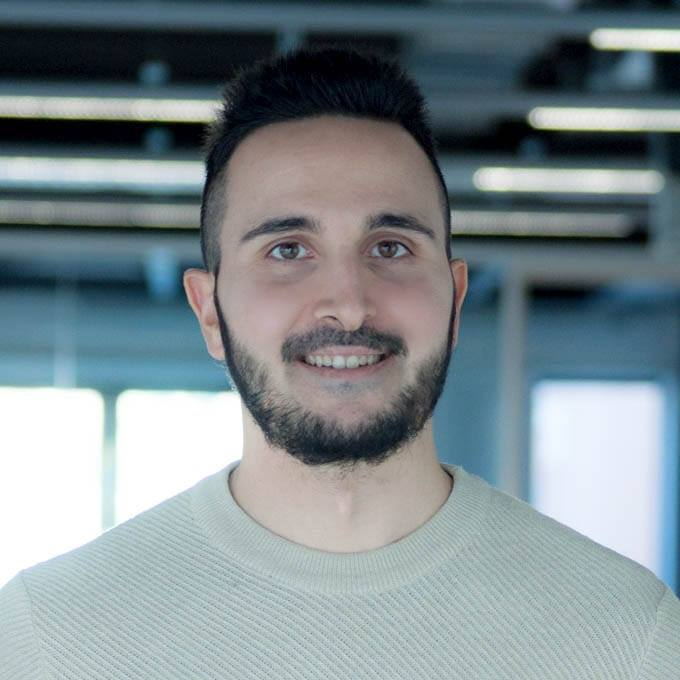
\includegraphics[width=13em]{me.jpg}}
\end{picture}


\hspace{24em}
\begin{minipage}[t]{0.4\textwidth} % 40% of the page width for the introduction text
	\vspace{-\baselineskip} % Required for vertically aligning minipages
	\cvsecttitle{Who am I?}

	Enthusiastic software developer with a constant desire to grow and learn new things.
    I like to write readable, testable and maintainable code to build quality software.

\end{minipage}
\vspace{\baselineskip} % Whitespaces before bubbles
\vspace{\baselineskip}

\begin{center}
	\bubbles{ 6/Java, 5/Kotlin, 5/Spring, 4/Docker, 4/Kubernetes, 5/TDD,
	3/TypeS, 2/ReactJs, 3/NodeJs, 4/Sql, 2/Php }
\end{center}

%----------------------------------------------------------------------------------------
%	EXPERIENCE
%----------------------------------------------------------------------------------------

\cvsect{Experience}{maingray}

\begin{entrylist}
    \entry
		{7/2021 -- current}
		{Senior Software engineer}
		{Friday Insurance SA - Berlin (Germany)}
		{Implementation of MyFriday area and related self-services.\\
        \texttt{Java}\slashsep\texttt{Kotlin}
        \slashsep\texttt{Docker}\slashsep\texttt{Kubernetes}
        \slashsep\texttt{Gitlab}\slashsep\texttt{Typescript}\slashsep\texttt{ReactJs}}
	\entry
		{2/2019 -- 5/2021}
		{Software engineer}
		{Dos Group SA - Mendrisio (Switzerland)}
		{Development of Comunemio for municipalities of canton of Ticino and its back-office platform.

        Contributing to an IoT system for tracking via Lora devices and to an application used by Swiss casinos for managing player's responsible gaming limits.

        Development of a web application for internal use for a Swiss television broadcaster.\\
        \texttt{Java}\slashsep\texttt{Spring}\slashsep\texttt{Kotlin}
        \slashsep\texttt{Docker}\slashsep\texttt{Kubernetes}
        \slashsep\texttt{Jenkins}\slashsep\texttt{Typescript}\\
        \texttt{Microservices}\slashsep\texttt{ReactJs}\slashsep\texttt{RabbitMq}
        \slashsep\texttt{Php}}
	\entry
		{11/2017 -- 1/2019}
		{Web developer}
		{Restart38 - Pavia (Italy)}
		{Development of the backend of various web applications for different customers.
		\\ \texttt{Java}\slashsep\texttt{Php}\slashsep\texttt{Javascript}}
	\entry
		{5/2016 -- 10/2017}
		{Software Developer}
		{eWitness - Milano (Italy)}
		{Implementation of solutions for the import and the secure archiving of documents to support companies in the dematerialization process.
        Maintenance of the eWitness digital archiving system and development of small functionalities of a MEAN web application.\\
        \texttt{Java}\slashsep\texttt{Mysql}\slashsep\texttt{AngularJs}
        \slashsep\texttt{Nodejs}\slashsep\texttt{Javascript}\slashsep\texttt{MongoDB}
        \slashsep\texttt{Linux}}
	\entry
		{6/2015 -- 9/2015\\\footnotesize{Internship for BSc}}
		{Junior Web Developer}
		{Elmec Informatica - Varese (Italy)}
		{Updating and adding new features to the company e-learning platform based on Moodle.\\
        \texttt{PHP}\slashsep\texttt{Javascript}\slashsep\texttt{Moodle}\slashsep\texttt{Linux}}
	\entry
		{11/2013 -- 1/2014\\\footnotesize{part time}}
		{Junior Help Desk}
		{lastminute.com - Chiasso (Switzerland)}
		{Supporting with mail server migration during studies at University.}
\end{entrylist}

%----------------------------------------------------------------------------------------
%	EDUCATION
%----------------------------------------------------------------------------------------

\cvsect{Education}{mainblue}

\begin{entrylist}
	\entry
		{2012 -- 2015}
		{Bachelor's Degree in Computer Science}
		{Università degli studi dell'Insubria - Varese (Italy)}
		{}
\end{entrylist}

%----------------------------------------------------------------------------------------
%	ADDITIONAL INFORMATION
%----------------------------------------------------------------------------------------

\begin{minipage}[t]{0.3\textwidth}
	\vspace{-\baselineskip} % Required for vertically aligning minipages

	\cvsect{Languages}{maingray}

	\textbf{Italian} - native\\
	\textbf{English} - proficient\\
	\textbf{French} - beginner
\end{minipage}
\hfill
\begin{minipage}[t]{0.3\textwidth}
	\vspace{-\baselineskip} % Required for vertically aligning minipages

	\cvsect{Hobbies}{mainblue}

	I like to play music and shoot some picture in my free time. I love to travel and visit new places.
\end{minipage}
\hfill
\begin{minipage}[t]{0.3\textwidth}
	\vspace{-\baselineskip} % Required for vertically aligning minipages

	\cvsect{Buzzwords}{maingray}

	Clean Code, TDD, Agile Software Development, Backend,\\
	Pair Programming, Maintainability, Code Readability
\end{minipage}

%----------------------------------------------------------------------------------------

\end{document}
